% HIGH-LEVEL sequence diagram (6 lanes). Detailed: sequence-detailed.tex
% Build:  cd docs/diagrams && pdflatex sequence-overview.tex && pdftoppm -png -r 144 -singlefile sequence-overview.pdf sequence-overview
\documentclass[tikz,border=14pt]{standalone}
\usepackage[scaled]{helvet}
\renewcommand\familydefault{\sfdefault}
\usepackage[T1]{fontenc}
\usetikzlibrary{arrows.meta,positioning,calc}

\definecolor{ink}{HTML}{1F2328}
\definecolor{muted}{HTML}{59636E}
\definecolor{rule}{HTML}{D0D7DE}
\definecolor{head}{HTML}{F6F8FA}
\definecolor{start}{HTML}{DAFBE1}   \definecolor{startline}{HTML}{1A7F37}
\definecolor{fault}{HTML}{FFEBE9}   \definecolor{faultline}{HTML}{CF222E}
\definecolor{rca}{HTML}{DDF4FF}     \definecolor{rcaline}{HTML}{0969DA}
\definecolor{heal}{HTML}{FBEFFF}    \definecolor{healline}{HTML}{8250DF}
\definecolor{note}{HTML}{FFF8C5}    \definecolor{noteline}{HTML}{D4A72C}

\newcommand{\lanegap}{3.9}
\newcommand{\rowh}{0.62}
% lane index -> x
\newcommand{\X}[1]{#1*\lanegap}
% \msg{from}{to}{row}{label}         request (solid)
% \rep{from}{to}{row}{label}         reply (dashed)
\newcommand{\msg}[4]{%
  \draw[-{Stealth[length=2.2mm]}, ink, line width=0.55pt] ({\X{#1}},{-#3*\rowh}) -- ({\X{#2}},{-#3*\rowh})
    node[midway, above=0.5pt, font=\scriptsize, text=ink, fill=white, fill opacity=0.9, text opacity=1, inner sep=1.2pt, align=center] {#4};}
\newcommand{\rep}[4]{%
  \draw[-{Stealth[length=2.2mm,open]}, muted, dashed, line width=0.5pt] ({\X{#1}},{-#3*\rowh}) -- ({\X{#2}},{-#3*\rowh})
    node[midway, above=0.5pt, font=\scriptsize, text=muted, fill=white, fill opacity=0.9, text opacity=1, inner sep=1.2pt, align=center] {#4};}
% \note{lane}{row}{text}
\newcommand{\note}[3]{%
  \node[draw=noteline, fill=note, rounded corners=1.5pt, font=\scriptsize, text=ink, inner sep=2.5pt,
        align=center] at ({\X{#1}},{-#2*\rowh}) {#3};}
% \phase{top row}{bottom row}{fill}{line}{title}
\newcommand{\phase}[5]{%
  \fill[#3] ({-1.55},{-#1*\rowh+0.34}) rectangle ({\X{5}+1.55},{-#2*\rowh-0.36});
  \draw[#4, line width=1.4pt] ({-1.55},{-#1*\rowh+0.34}) -- ({-1.55},{-#2*\rowh-0.36});
  \node[anchor=north west, font=\footnotesize\bfseries, text=#4] at ({-1.45},{-#1*\rowh+0.30}) {#5};}

\begin{document}
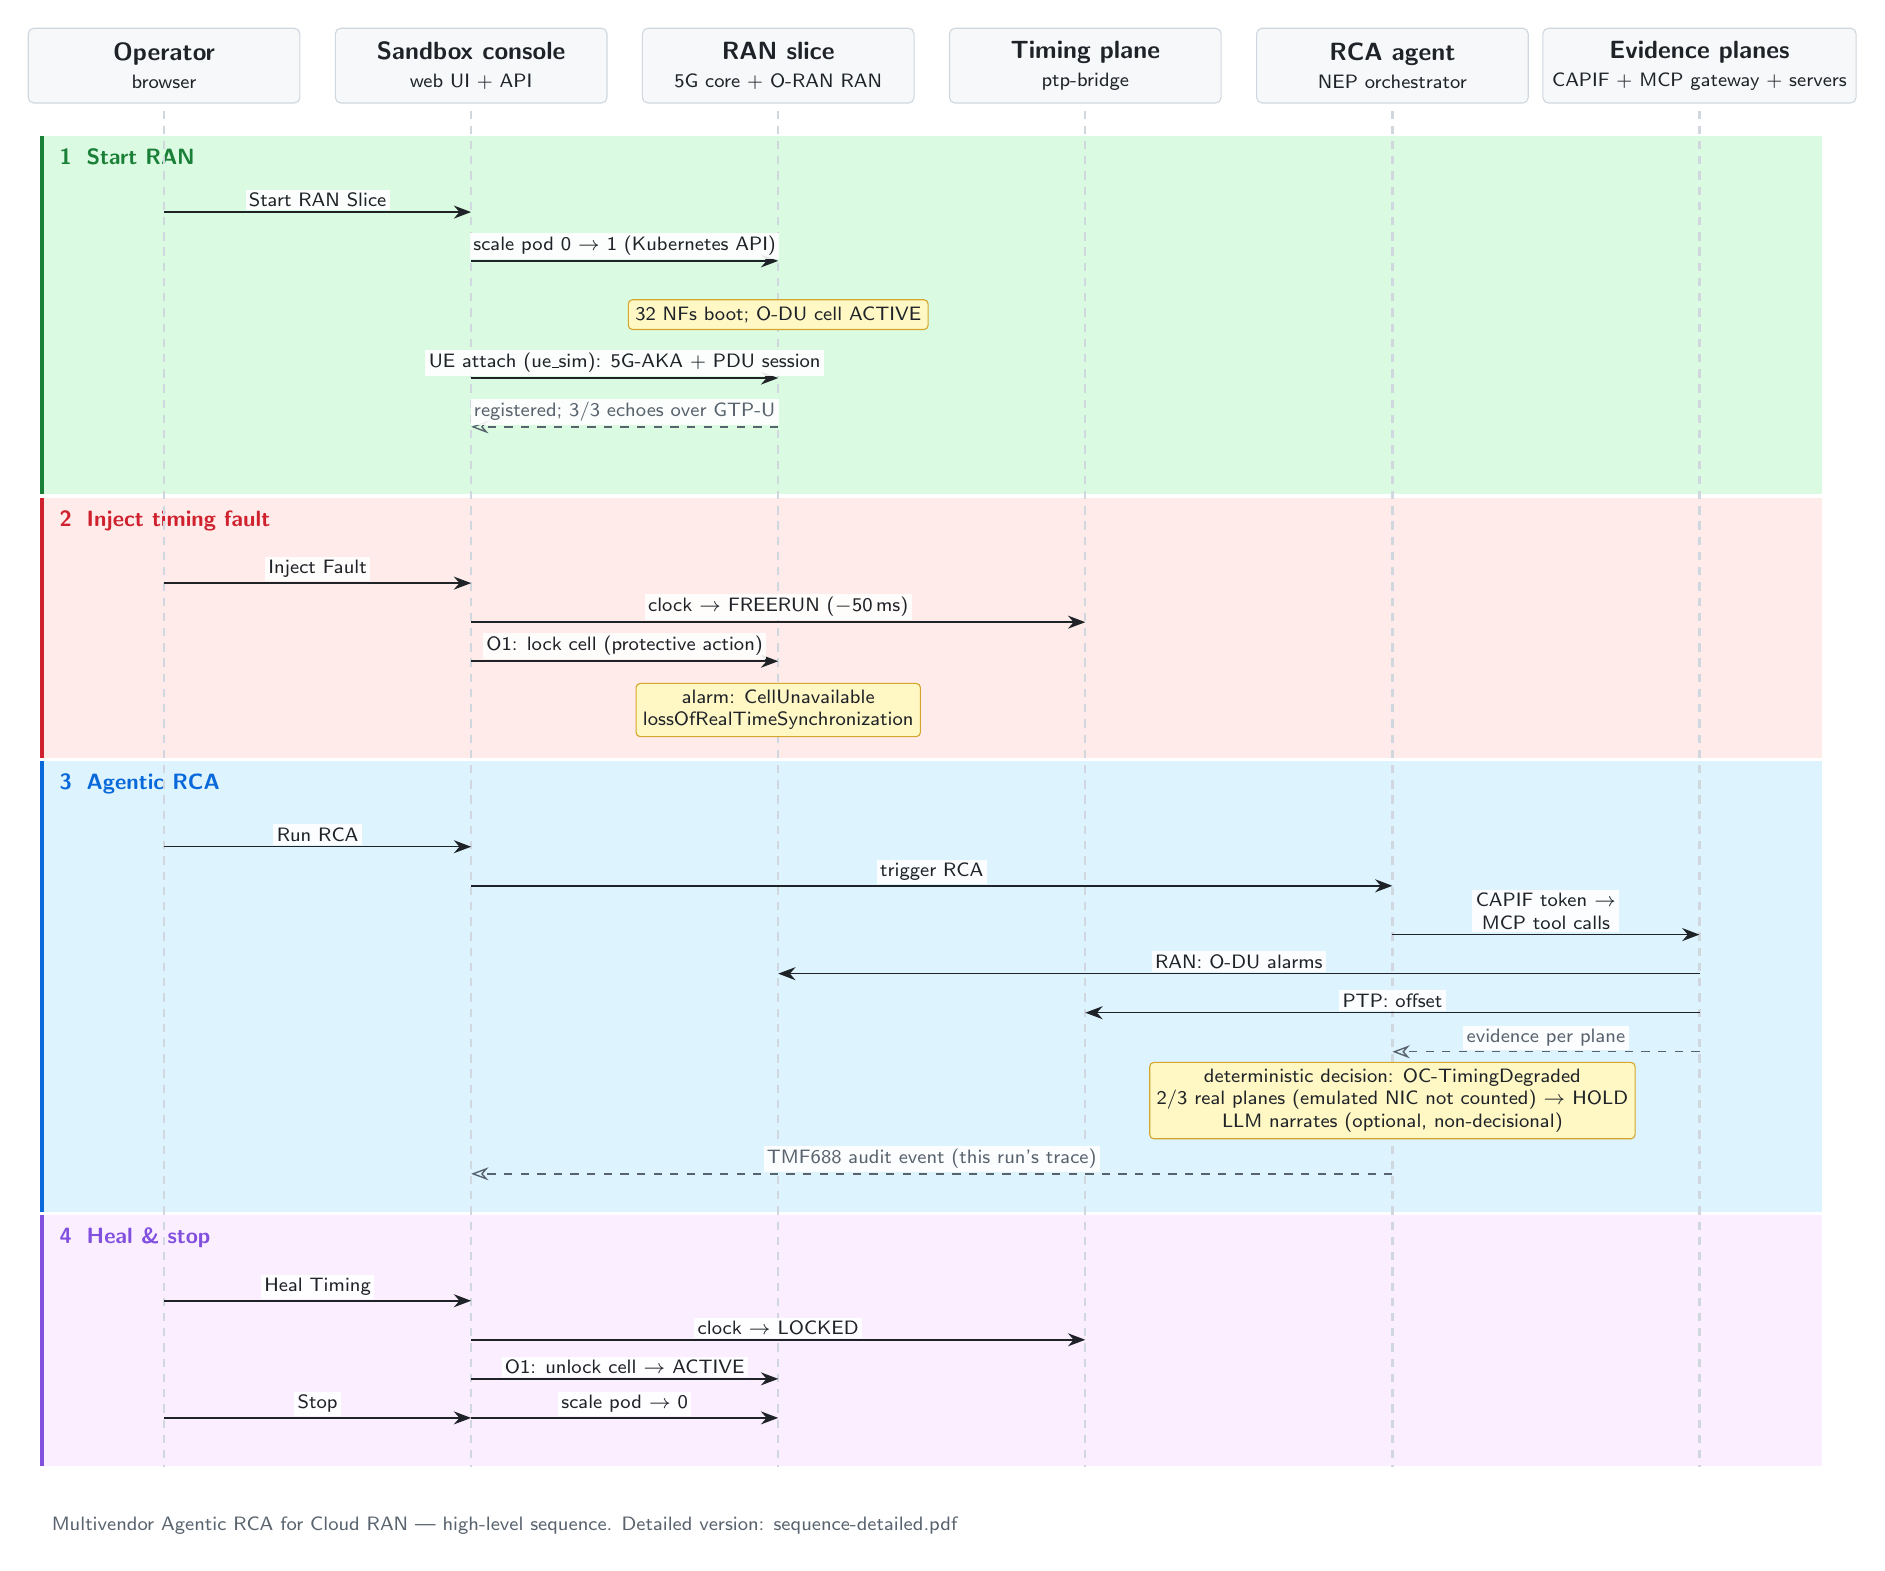
\begin{tikzpicture}[x=1cm,y=1cm]

\phase{1}{7.2}{start}{startline}{1 \;Start RAN}
\phase{8.4}{12.6}{fault}{faultline}{2 \;Inject timing fault}
\phase{13.8}{21.9}{rca}{rcaline}{3 \;Agentic RCA}
\phase{23.1}{27.1}{heal}{healline}{4 \;Heal \& stop}

\foreach \i/\name in {0/{Operator\\[-1pt]\scriptsize\mdseries browser},
                      1/{Sandbox console\\[-1pt]\scriptsize\mdseries web UI + API},
                      2/{RAN slice\\[-1pt]\scriptsize\mdseries 5G core + O-RAN RAN},
                      3/{Timing plane\\[-1pt]\scriptsize\mdseries ptp-bridge},
                      4/{RCA agent\\[-1pt]\scriptsize\mdseries NEP orchestrator},
                      5/{Evidence planes\\[-1pt]\scriptsize\mdseries CAPIF + MCP gateway + servers}} {
  \draw[rule, line width=0.8pt, dash pattern=on 3pt off 2.5pt] ({\X{\i}},0.05) -- ({\X{\i}},{-27.7*\rowh});
  \node[draw=rule, fill=head, rounded corners=2pt, minimum width=3.45cm, minimum height=0.95cm,
        align=center, font=\small\bfseries, text=ink] at ({\X{\i}},0.62) {\name};
}

% 1. Start
\msg{0}{1}{2}{Start RAN Slice}
\msg{1}{2}{3}{scale pod 0 $\to$ 1 (Kubernetes API)}
\note{2}{4.1}{32 NFs boot; O-DU cell ACTIVE}
\msg{1}{2}{5.4}{UE attach (ue\_sim): 5G-AKA + PDU session}
\rep{2}{1}{6.4}{registered; 3/3 echoes over GTP-U}

% 2. Fault
\msg{0}{1}{9.6}{Inject Fault}
\msg{1}{3}{10.4}{clock $\to$ FREERUN ($-$50\,ms)}
\msg{1}{2}{11.2}{O1: lock cell (protective action)}
\note{2}{12.2}{alarm: CellUnavailable\\lossOfRealTimeSynchronization}

% 3. RCA
\msg{0}{1}{15}{Run RCA}
\msg{1}{4}{15.8}{trigger RCA}
\msg{4}{5}{16.8}{CAPIF token $\to$\\MCP tool calls}
\msg{5}{2}{17.6}{RAN: O-DU alarms}
\msg{5}{3}{18.4}{PTP: offset}
\rep{5}{4}{19.2}{evidence per plane}
\note{4}{20.2}{deterministic decision: OC-TimingDegraded\\2/3 real planes (emulated NIC not counted) $\to$ HOLD\\LLM narrates (optional, non-decisional)}
\rep{4}{1}{21.7}{TMF688 audit event (this run's trace)}

% 4. Heal & stop
\msg{0}{1}{24.3}{Heal Timing}
\msg{1}{3}{25.1}{clock $\to$ LOCKED}
\msg{1}{2}{25.9}{O1: unlock cell $\to$ ACTIVE}
\msg{0}{1}{26.7}{Stop}
\draw[-{Stealth[length=2.2mm]}, ink, line width=0.55pt] ({\X{1}},{-26.7*\rowh}) -- ({\X{2}},{-26.7*\rowh})
  node[midway, above=0.5pt, font=\scriptsize, fill=white, fill opacity=0.9, text opacity=1, inner sep=1.2pt] {scale pod $\to$ 0};

\node[anchor=west, font=\scriptsize, text=muted] at (-1.55,{-28.9*\rowh})
  {Multivendor Agentic RCA for Cloud RAN — high-level sequence. Detailed version: sequence-detailed.pdf};

\end{tikzpicture}
\end{document}
